% ============================================================
%  GP Hybrid: Mentor Meeting Summary  (4 slides)
%  Compile: pdflatex gp_hybrid_summary_slides.tex  (run twice)
%  Requires: beamer-theme-metropolis
% ============================================================
\documentclass[aspectratio=169, 10pt]{beamer}

\usetheme{metropolis}

% ── packages ────────────────────────────────────────────────
\usepackage{booktabs}
\usepackage{amsmath, amssymb}
\usepackage{graphicx}
\usepackage{xcolor}
\usepackage{tikz}
\usepackage[protrusion=true, expansion=false]{microtype}
\usepackage[T1]{fontenc}
\usetikzlibrary{arrows.meta, positioning, shapes.geometric, fit,
                backgrounds, calc, decorations.pathreplacing}

\graphicspath{{./}{../hybrid_qoz_experiment/results_b2/}}

% ── colour palette ──────────────────────────────────────────
\definecolor{cnavy}{HTML}{0D2137}
\definecolor{cteal}{HTML}{1A6B8A}
\definecolor{cmint}{HTML}{02C39A}
\definecolor{cice}{HTML}{E4F2F8}
\definecolor{cmid}{HTML}{7BB8CC}
\definecolor{cdgray}{HTML}{2E4057}
\definecolor{camber}{HTML}{F0A500}
\definecolor{cmuted}{HTML}{5A7385}
\definecolor{cred}{HTML}{E05C5C}

% ── metropolis overrides ────────────────────────────────────
\setbeamercolor{normal text}{fg=cnavy, bg=white}
\setbeamercolor{frametitle}{bg=cnavy, fg=white}
\setbeamercolor{title separator}{fg=cmint}
\setbeamercolor{progress bar}{fg=cmint, bg=cice}
\setbeamercolor{alerted text}{fg=cmint}
\setbeamercolor{block title}{bg=cice, fg=cnavy}
\setbeamercolor{block body}{bg=cice!40, fg=cnavy}
\setbeamercolor{itemize item}{fg=cteal}
\setbeamercolor{itemize subitem}{fg=cmuted}
\setbeamerfont{frametitle}{size=\large, series=\bfseries}
\setbeamerfont{block title}{series=\bfseries, size=\footnotesize}
\setbeamerfont{block body}{size=\footnotesize}

\setlength{\parskip}{2pt}

% ── title info ───────────────────────────────────────────────
\title{GP-Assisted Dyadic Compression}
\subtitle{Progress Summary}
\author{Jessie Chen}
\institute{Argonne National Laboratory}
\date{October 2026}

% ─────────────────────────────────────────────────────────────
\begin{document}

% ══════════════════════════════════════════════════════════════
% SLIDE 1: Dyadic Grid in QoZ / SZ3
% ══════════════════════════════════════════════════════════════
\begin{frame}{Dyadic Grid Refinement in QoZ / SZ3}

\begin{columns}[T, totalwidth=\textwidth]
% ── left: text ───────────────────────────────────────────────
\begin{column}{0.44\textwidth}
  {\footnotesize
  \textbf{QoZ} and \textbf{SZ3} with \texttt{ALGO\_INTERP} use a
  \textbf{dyadic (halving) refinement} schedule to predict data values
  hierarchically.

  \medskip
  \begin{itemize}\setlength\itemsep{3pt}
    \item[\textcolor{cnavy}{\textbullet}]
      \textbf{Level 0} — coarsest grid\\
      {\scriptsize Points spaced at initial stride (e.g.\ 32).\\
       Stored as raw floats — no prediction.}
    \item[\textcolor{cteal}{\textbullet}]
      \textbf{Level 1} — halved stride\\
      {\scriptsize Midpoints predicted by cubic spline\\
       interpolation from Level 0 anchors.}
    \item[\textcolor{cmid}{\textbullet}]
      \textbf{Level 2+} — repeat halving\\
      {\scriptsize Each level predicts from the previous,\\
       recursively refining the grid.}
  \end{itemize}

  \medskip
  {\scriptsize\color{cmuted}
  Prediction residuals are quantized and entropy-coded\\
  (Huffman + zstd).  Anchor points dominate the bit budget\\
  at low error bounds.}
  }
\end{column}

% ── right: 2D TikZ dyadic grid ───────────────────────────────
\begin{column}{0.54\textwidth}
\centering
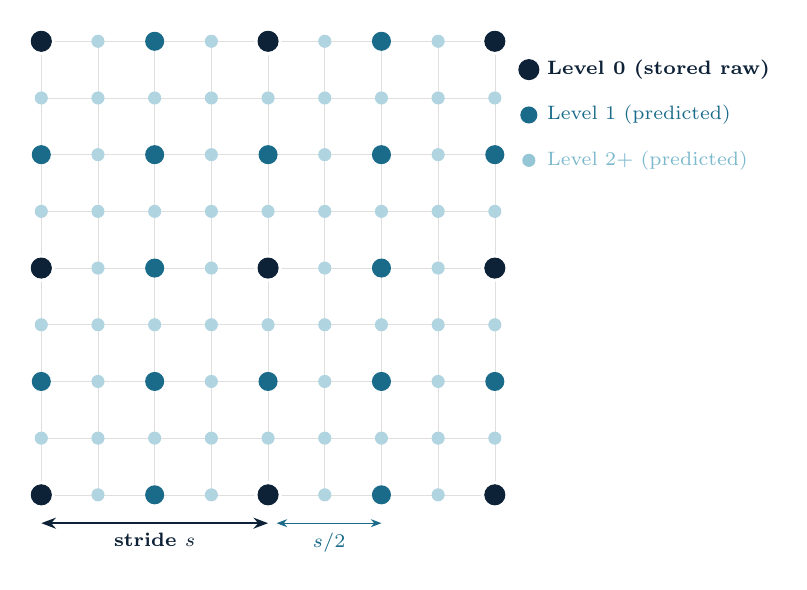
\begin{tikzpicture}[scale=0.72]
  % ── grid lines (faint) ──────────────────────────────────
  \draw[gray!25, very thin, step=1] (0,0) grid (8,8);

  % ── L2 midpoints (small, light) ─────────────────────────
  \foreach \x in {1,3,5,7}{
    \foreach \y in {0,2,4,6,8}{
      \filldraw[cmid!60] (\x,\y) circle (3pt);
    }
  }
  \foreach \x in {0,2,4,6,8}{
    \foreach \y in {1,3,5,7}{
      \filldraw[cmid!60] (\x,\y) circle (3pt);
    }
  }
  \foreach \x in {1,3,5,7}{
    \foreach \y in {1,3,5,7}{
      \filldraw[cmid!60] (\x,\y) circle (3pt);
    }
  }

  % ── L1 midpoints (medium, teal) ─────────────────────────
  \foreach \x in {2,6}{
    \foreach \y in {0,4,8}{
      \filldraw[cteal] (\x,\y) circle (4.5pt);
    }
  }
  \foreach \x in {0,4,8}{
    \foreach \y in {2,6}{
      \filldraw[cteal] (\x,\y) circle (4.5pt);
    }
  }
  \filldraw[cteal] (2,2) circle (4.5pt);
  \filldraw[cteal] (6,2) circle (4.5pt);
  \filldraw[cteal] (2,6) circle (4.5pt);
  \filldraw[cteal] (6,6) circle (4.5pt);

  % ── L0 anchors (large, navy) ────────────────────────────
  \foreach \x in {0,4,8}{
    \foreach \y in {0,4,8}{
      \filldraw[cnavy] (\x,\y) circle (6pt);
      \draw[white, very thick] (\x,\y) circle (6pt);
      \filldraw[cnavy] (\x,\y) circle (5pt);
    }
  }

  % ── brace annotations ───────────────────────────────────
  \draw[{Stealth[scale=0.8]}-{Stealth[scale=0.8]}, cnavy, thick]
    (0,-0.5) -- (4,-0.5) node[midway, below, font=\scriptsize\bfseries] {stride $s$};
  \draw[{Stealth[scale=0.8]}-{Stealth[scale=0.8]}, cteal]
    (4.15,-0.5) -- (6.0,-0.5) node[midway, below, font=\scriptsize] {$s/2$};

  % ── legend (right of grid) ──────────────────────────────
  \begin{scope}[xshift=8.6cm]
    \filldraw[cnavy] (0,7.5) circle (5pt);
    \node[right, font=\scriptsize\bfseries, text=cnavy] at (0.15,7.5) {Level 0 (stored raw)};

    \filldraw[cteal] (0,6.7) circle (4pt);
    \node[right, font=\scriptsize, text=cteal] at (0.15,6.7) {Level 1 (predicted)};

    \filldraw[cmid!80] (0,5.9) circle (3pt);
    \node[right, font=\scriptsize, text=cmid] at (0.15,5.9) {Level 2+ (predicted)};
  \end{scope}
\end{tikzpicture}
\end{column}
\end{columns}

\end{frame}

% ══════════════════════════════════════════════════════════════
% SLIDE 2: GP Pre-Pass — GKS Anchor Selection
% ══════════════════════════════════════════════════════════════
\begin{frame}{GP Pre-Pass: Replacing Cubic Splines at L0/L1}

\begin{columns}[T, totalwidth=\textwidth]
% ── left: explanation ────────────────────────────────────────
\begin{column}{0.44\textwidth}
  {\footnotesize
  \textbf{Why a GP instead of a cubic spline?}\\[2pt]
  {\scriptsize
  At L0/L1, anchor points can be \emph{far apart} (stride\,=\,32+).
  Cubic splines use only the \textbf{nearest 4 neighbors} — they
  extrapolate poorly across large gaps and cannot exploit smooth
  global structure.

  A GP with a stationary kernel (e.g.\ Matérn-$\tfrac{5}{2}$)
  conditions on \emph{all} stored anchors simultaneously, producing
  a posterior mean that remains accurate even when the prediction
  point is far from every anchor.  It also degrades gracefully:
  uncertainty ($\sigma$) grows with distance, while the mean
  still exploits the global covariance structure.}

  \medskip
  \textbf{GKS anchor selection}~\cite{GKS}:\\[2pt]
  {\scriptsize Greedy algorithm: pick the subset of L0 grid points
  that minimizes worst-case GP posterior variance over the domain.
  Those points are stored at \emph{full precision}; all others
  are predicted.}

  \medskip
  \begin{itemize}\setlength\itemsep{2pt}
    \item[\textcolor{camber}{\textbullet}]
      \textbf{GKS anchors} — stored raw\\
      {\scriptsize GP training inputs; $\sigma\!=\!0$ here.}
    \item[\textcolor{cmint}{\textbullet}]
      \textbf{Remaining L0/L1 pts} — GP-predicted\\
      {\scriptsize Posterior mean, better than spline far from anchors.}
    \item[\textcolor{cmid!80}{\textbullet}]
      \textbf{L2+} — cubic spline (unchanged from QoZ/SZ3)
  \end{itemize}
  }
\end{column}

% ── right: annotated dyadic grid ─────────────────────────────
\begin{column}{0.54\textwidth}
\centering
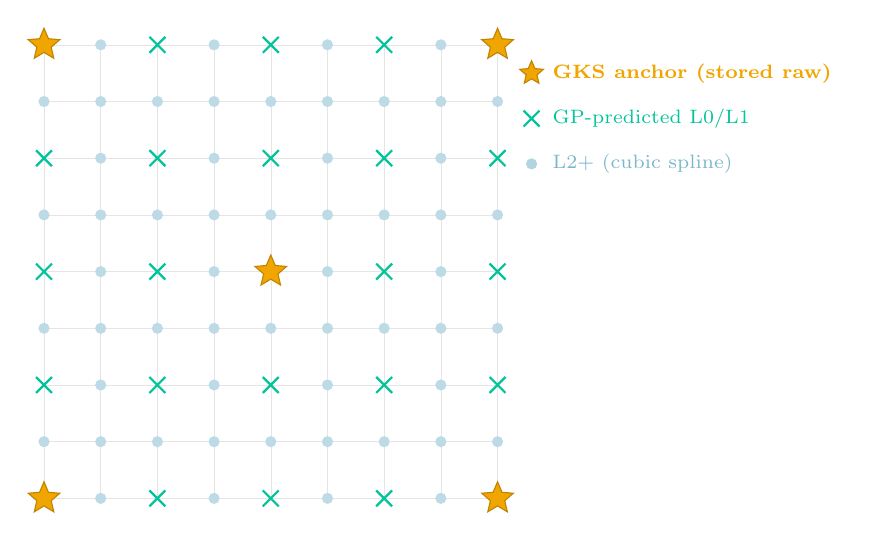
\begin{tikzpicture}[scale=0.72]
  % ── faint grid ──────────────────────────────────────────
  \draw[gray!20, very thin, step=1] (0,0) grid (8,8);

  % ── L2+ midpoints (small, gray) ─────────────────────────
  \foreach \x in {1,3,5,7}{
    \foreach \y in {0,2,4,6,8}{
      \filldraw[cmid!50] (\x,\y) circle (2.5pt);
    }
  }
  \foreach \x in {0,2,4,6,8}{
    \foreach \y in {1,3,5,7}{
      \filldraw[cmid!50] (\x,\y) circle (2.5pt);
    }
  }
  \foreach \x in {1,3,5,7}{
    \foreach \y in {1,3,5,7}{
      \filldraw[cmid!50] (\x,\y) circle (2.5pt);
    }
  }

  % ── GP-predicted L0/L1 (cmint diamonds) ─────────────────
  % L1 midpoints (non-GKS L0/L1 → GP predicted)
  \foreach \x/\y in {2/0, 6/0, 0/2, 4/2, 8/2, 2/4, 6/4, 0/6, 4/6, 8/6, 2/8, 6/8,
                     2/2, 6/2, 2/6, 6/6}{
    \draw[cmint, thick] (\x,\y) +(-4pt,-4pt) -- +(4pt,4pt)
                                +(4pt,-4pt)  -- +(-4pt,4pt);
  }
  % some L0 pts also GP-predicted (non-GKS)
  \foreach \x/\y in {4/0, 0/4, 8/4, 4/8}{
    \draw[cmint, thick] (\x,\y) +(-4pt,-4pt) -- +(4pt,4pt)
                                +(4pt,-4pt)  -- +(-4pt,4pt);
  }

  % ── GKS-selected anchors (camber stars) ─────────────────
  \foreach \x/\y in {0/0, 8/0, 0/8, 8/8, 4/4}{
    \node[star, star points=5, star point ratio=2.2,
          fill=camber, draw=camber!80!black, minimum size=12pt,
          inner sep=0pt] at (\x,\y) {};
  }

  % ── legend ──────────────────────────────────────────────
  \begin{scope}[xshift=8.6cm]
    \node[star, star points=5, star point ratio=2.2,
          fill=camber, draw=camber!80!black, minimum size=9pt,
          inner sep=0pt] at (0,7.5) {};
    \node[right, font=\scriptsize\bfseries, text=camber] at (0.2,7.5)
      {GKS anchor (stored raw)};

    \draw[cmint, thick] (0,6.7) +(-4pt,-4pt) -- +(4pt,4pt)
                                +(4pt,-4pt)  -- +(-4pt,4pt);
    \node[right, font=\scriptsize, text=cmint] at (0.2,6.7)
      {GP-predicted L0/L1};

    \filldraw[cmid!60] (0,5.9) circle (2.5pt);
    \node[right, font=\scriptsize, text=cmid] at (0.2,5.9)
      {L2+ (cubic spline)};
  \end{scope}
\end{tikzpicture}

{\scriptsize\color{cmuted}
\textbf{Savings}: fewer stored anchors $\Rightarrow$ smaller header;
GP captures smooth spatial structure missed by local splines.}
\end{column}
\end{columns}

% ── bibliography entry ───────────────────────────────────────
\vspace{2pt}
{\tiny\color{cmuted}
[GKS] \url{https://arxiv.org/abs/2601.20781}}

\end{frame}

% ══════════════════════════════════════════════════════════════
% SLIDE 3: GP Uncertainty Quantification
% ══════════════════════════════════════════════════════════════
\begin{frame}{Quantified Uncertainty in GP-Predicted Anchors}

\begin{columns}[T, totalwidth=\textwidth]
% ── left: key points ─────────────────────────────────────────
\begin{column}{0.42\textwidth}
  {\footnotesize
  Unlike cubic splines, a GP returns not only a \textbf{posterior mean}
  $\mu(x)$ but also a \textbf{posterior variance} $\sigma^2(x)$ at
  every predicted point.

  \medskip
  \begin{itemize}\setlength\itemsep{4pt}
    \item[\textcolor{camber}{\textbullet}]
      \textbf{Anchor points} (GKS) fix $\sigma\!=\!0$\\
      {\scriptsize GP is conditioned on these; uncertainty collapses.}
    \item[\textcolor{cmint}{\textbullet}]
      \textbf{Predicted anchors} carry $\sigma(x)$\\
      {\scriptsize Uncertainty grows between stored anchors and\\
       shrinks near them — shown right.}
    \item[\textcolor{cteal}{\textbullet}]
      \textbf{Adaptive quantization}\\
      {\scriptsize $\sigma$ can guide EB allocation: tighter bounds\\
       where the GP is uncertain, looser where it is confident.}
  \end{itemize}

  \medskip
  \begin{block}{\scriptsize Potential use}
    {\scriptsize
    Rate–distortion optimization: allocate more bits at high-$\sigma$
    predicted anchors, fewer bits at low-$\sigma$ ones, without
    violating the global error bound.}
  \end{block}
  }
\end{column}

% ── right: TikZ GP posterior illustration ────────────────────
\begin{column}{0.56\textwidth}
\centering
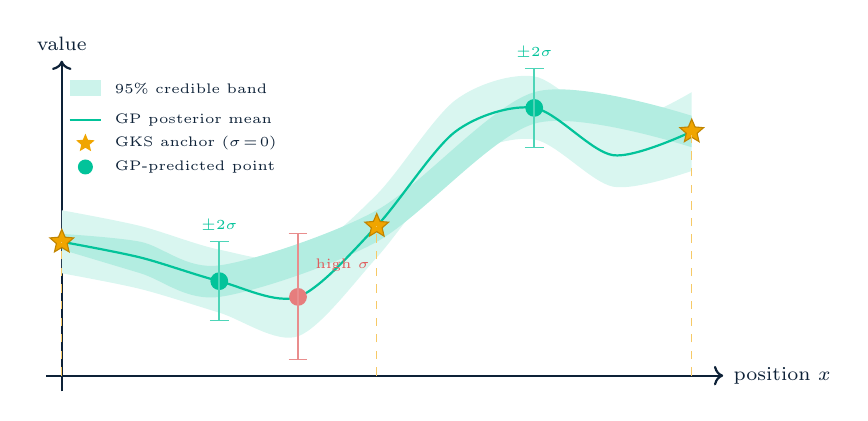
\begin{tikzpicture}[scale=1.0]
  % axes
  \draw[->, thick, cnavy] (-0.2,0) -- (8.4,0) node[right, font=\scriptsize] {position $x$};
  \draw[->, thick, cnavy] (0,-0.2) -- (0,4.0) node[above, font=\scriptsize] {value};

  % ── confidence band (±2σ) ──────────────────────────────
  \fill[cmint!15]
    plot[smooth, tension=0.5] coordinates
      {(0,1.3)(1,1.1)(2,0.8)(3,0.5)(4,1.5)(5,2.7)(6,3.0)(7,2.4)(8,2.6)}
    -- plot[smooth, tension=0.5] coordinates
      {(8,3.6)(7,3.2)(6,3.8)(5,3.5)(4,2.3)(3,1.5)(2,1.6)(1,1.9)(0,2.1)}
    -- cycle;

  % ── tighter bands near anchors ─────────────────────────
  \fill[cmint!30]
    plot[smooth, tension=0.5] coordinates
      {(0,1.6)(1,1.3)(2,1.0)(4,1.7)(6,3.2)(8,2.9)}
    -- plot[smooth, tension=0.5] coordinates
      {(8,3.3)(6,3.6)(4,2.1)(2,1.4)(1,1.7)(0,1.8)}
    -- cycle;

  % ── GP posterior mean ──────────────────────────────────
  \draw[cmint, thick, smooth, tension=0.5]
    plot coordinates {(0,1.7)(1,1.5)(2,1.2)(3,1.0)(4,1.9)(5,3.1)(6,3.4)(7,2.8)(8,3.1)};

  % ── GKS anchors (conditioning points) ──────────────────
  \foreach \x/\y in {0/1.7, 4/1.9, 8/3.1}{
    \node[star, star points=5, star point ratio=2.2,
          fill=camber, draw=camber!80!black,
          minimum size=9pt, inner sep=0pt] at (\x,\y) {};
    \draw[camber!60, dashed, thin] (\x,0) -- (\x,\y);
  }

  % ── predicted L0/L1 pts with uncertainty bars ──────────
  \foreach \x/\ymid/\ylo/\yhi in {2/1.2/0.7/1.7, 6/3.4/2.9/3.9}{
    \filldraw[cmint] (\x,\ymid) circle (3pt);
    \draw[cmint!70, thick] (\x,\ylo) -- (\x,\yhi);
    \draw[cmint!70] (\x-0.12,\ylo) -- (\x+0.12,\ylo);
    \draw[cmint!70] (\x-0.12,\yhi) -- (\x+0.12,\yhi);
    \node[above, font=\tiny, text=cmint] at (\x,\yhi) {$\pm 2\sigma$};
  }

  % midpoint with larger uncertainty (far from anchor)
  \filldraw[cred!80] (3,1.0) circle (3pt);
  \draw[cred!70, thick] (3,0.2) -- (3,1.8);
  \draw[cred!70] (2.88,0.2) -- (3.12,0.2);
  \draw[cred!70] (2.88,1.8) -- (3.12,1.8);
  \node[right, font=\tiny, text=cred] at (3.1,1.4) {high $\sigma$};

  % ── legend ─────────────────────────────────────────────
  \fill[cmint!20] (0.1,3.55) rectangle (0.5,3.75);
  \node[right, font=\tiny, text=cnavy] at (0.55,3.65) {95\% credible band};

  \draw[cmint, thick] (0.1,3.25) -- (0.5,3.25);
  \node[right, font=\tiny, text=cnavy] at (0.55,3.25) {GP posterior mean};

  \node[star, star points=5, star point ratio=2.2, fill=camber,
        minimum size=7pt, inner sep=0pt] at (0.3,2.95) {};
  \node[right, font=\tiny, text=cnavy] at (0.55,2.95) {GKS anchor ($\sigma\!=\!0$)};

  \filldraw[cmint] (0.3,2.65) circle (2.5pt);
  \node[right, font=\tiny, text=cnavy] at (0.55,2.65) {GP-predicted point};
\end{tikzpicture}
\end{column}
\end{columns}

\end{frame}

% ══════════════════════════════════════════════════════════════
% SLIDE 4: Hurricane ISABEL W — Results
% ══════════════════════════════════════════════════════════════
\begin{frame}{Hurricane ISABEL W — Rate-Distortion Results}

\begin{columns}[T, totalwidth=\textwidth]

\begin{column}{0.495\textwidth}
  \centering
  {\footnotesize\bfseries\color{cnavy} PSNR vs.\ Bit-rate}\\[3pt]
  \includegraphics[width=\linewidth, height=0.72\textheight,
                   keepaspectratio]{rd_b2.png}
\end{column}

\begin{column}{0.01\textwidth}\end{column}   % thin spacer

\begin{column}{0.495\textwidth}
  \centering
  {\footnotesize\bfseries\color{cnavy} SSIM vs.\ Bit-rate}\\[3pt]
  \includegraphics[width=\linewidth, height=0.72\textheight,
                   keepaspectratio]{ssim_b2.png}
\end{column}

\end{columns}

\vspace{2pt}
{\scriptsize\color{cmuted}
Dataset: Hurricane ISABEL \texttt{Wf48} ($100\!\times\!500\!\times\!500$ f32).
GP-QoZ: stride\,=\,32, \texttt{gp\_levels}\,=\,2, Huffman\,+\,zstd.
\textbf{Labels next to each point} show the relative error bound $\varepsilon$ tested at that setting
($\varepsilon \in \{10^{-2},\,5\!\times\!10^{-3},\,10^{-3},\,5\!\times\!10^{-4},\,10^{-4}\}$;
smaller $\varepsilon$ = tighter bound = higher bit-rate).}

\end{frame}

\end{document}
